\chapter{Materiales y métodos}
En este capítulo se describe cómo fueron realizadas las simulaciones de los campos gaussianos aleatorios para poder ser replicadas. También se especifican los materiales que fueron usados durante todo el proceso.

Se generaron realizaciones tridimensionales (de las que se tomaron cortes bidimensionales), así como una visualización animada de la tercera dimensión en formato GIF o MP4, del campo de fluctuaciones gaussiano para ambos espectros de potencias y diferentes valores de \(n_s\). En primer lugar para el espectro de potencias primordial \(\symrm{P}_0(k)\):
\begin{itemize}
    \item \(n_s=0\). Ruido blanco, el fondo sobre el que se perturba. Sirvió para comprobar el funcionamiento.
    \item \(n_s=1\). Harrison-Zel'dovich. Grandes escalas, se utilizó para comprobar un espectro \textit{blue-tilted} que se refiere a un espectro donde las longitudes de onda pequeñas (azul) fluctúan más, es decir, fluctuaciones de menor tamaño físico.
    \item \(n_s=-3\). Pequeñas escalas del universo, sirvió para comprobar un espectro \textit{red-tilted} que es la contraparte del anterior, donde las longitudes de onda largas (rojo) fluctúan más, es decir, fluctuaciones de mayor tamaño físico.
\end{itemize}
Y al final, para la simulación más realista se utilizó~\eqref{eq::espectrolineal} y~\eqref{eq::transff}:
\begin{itemize}
    \item \(n_s=5\). En este caso, \(P(k)\propto k\) que corresponde a grandes escalas y ha de ser homogéneo con pequeñas fluctuaciones.
    \item \(n_s=1\). Es equivalente a \(P(k)\propto k^{-3}\) que apunta a escalas más pequeñas donde las fluctuaciones son más grandes.
\end{itemize}

Como no es posible simular campos infinitos, se generaron muestras del verdadero campo subyacente, es decir, ``cajas'' que son representaciones periódicas del susodicho campo. En este aspecto las transformadas de Fourier~\eqref{eq::fourierinverse} y~\eqref{eq::fourier} se tornan discretas:\footnote{Para ahorrar notación se escribe la transformada discreta en una dimensión, la cual se extiende a mayores dimensiones de manera obvia.}
\begin{equation}
    \delta_m(k)\equiv\frac{1}{L}\sum_{n=0}^{N-1}\delta_n(x)\ \symrm{e}^{-\symrm{i}nm/N}=\frac{\mathcal{F}\left[\delta({x})\right]}{L}\qquad m=0,\ldots,n-1,\label{eq::discrete}
\end{equation}
donde \(L\) es el lado de la caja y \(N\) es la cantidad de números de onda \(k\) a utilizar (número de celdas en un lado de la caja), tal que para cada dimensión \((d=1,2,3)\) se usaron las condiciones de contorno periódicas habituales:
\begin{equation}
    k_d=\frac{2\pi}{L}j,\quad j\in\left(-\frac{N}{2},\ldots,\frac{N}{2}\right).\label{eq::knumbers}
\end{equation}
Para obtener un espectro de potencias cuya magnitud fuese independiente del volumen de la propia caja se normalizó por volumen en la transformada discreta tridimensional extendida de~\eqref{eq::discrete}, por lo que se se tuvo que normalizar el espectro de potencias:
\begin{equation}
    \tilde{\symrm{P}}(k)=\frac{\symrm{P}(k)}{L^3},
\end{equation}
donde \(\tilde{\symrm{P}}(k)\) tiene unidades \([x]^3\equiv[k]^{-3}\). El valor \(L\) indica cuanta distancia física representa 1 píxel:
\begin{equation}
    [L]=\frac{[x]}{[\symrm{p\acute{\imath}xel}]}.
\end{equation}
Usando diferentes valores de \(L\) se pudieron simular zonas del universo de distintos tamaños y, observar cómo variaba el campo de fluctuaciones de la densidad \(\delta(\symbf{x})\).
\section{Método}
El algoritmo (véase~\autoref{ch::codes}) se implementó con el lenguaje de programación Python con gran soporte de la librería Numpy~\cite{harris2020array} y Powerbox~\cite{Murray2018}. Los pasos lógicos son los siguientes:
\begin{enumerate}
    \item Dada una caja de longitud \(L\) (parámetro \texttt{boxlength}) y número de celdas a lo largo de un lado, \(N\) (parámetro \texttt{self.\_size}), se determinan los números de onda \(k\) a lo largo de este lado de acuerdo a~\eqref{eq::knumbers}.
    \item A partir de estos números de onda a lo largo de cada lado se determinan sus magnitudes en todos los puntos de la caja tridimensional, lo que da lugar al \textit{array} de los números de onda \(k_j=\sqrt{\sum_d k^2_{d,j}}\) de dimensiones \(N\times N\times N\).
    \item Se crea el \textit{array} del campo aleatorio gaussiano de media nula y desviación típica unitaria, \(G\), cuyas dimensiones han de ser \(N\times N\times N\), el cual asigna de forma aleatoria un número complejo a cada punto del mallado tridimensional. El número complejo tendrá módulo tomado de \(\mathcal{N}(0,1)\) y la fase de \(U(0,2\pi)\).
    \item Se calcula el \textit{array} del espectro de potencias \(\symrm{P}(k_j)\) pasando \(k_j\) por una función que represente a~\eqref{eq::espectroprim} o~\eqref{eq::espectrolineal}.
    \item Se computa el \textit{array} del campo de fluctuaciones en el espacio de Fourier \(\delta(\symbf{k})=G\,\sqrt{\symrm{P}(k_j)}\). Se multiplica por la raíz de \(\symrm{P}(k_j)\) para pasar a desviación típica \(\symrm{P}(k)\).
    \item Se determina el campo de fluctuaciones en el espacio real mediante la transformada inversa de Fourier \(\delta(\symbf{x})=L^3\mathcal{F}^{-1}\left[\delta(\symbf{k})\right]\).
\end{enumerate}
El índice espectral \(n_s\) es el parámetro \texttt{power} y la amplitud del espectro de potencias lineal \(A_0\) es \texttt{amplitude} para \(k_0=0.05\) Mpc\textsuperscript{-1}. Al fijar \(k_0\) en estas unidades, la unidad de distancia física obtenida fue el megapársec, \([x]=\text{Mpc}\).

Para poder replicar los resultados que se obtuvieron, la semilla inicial que da lugar a los números aleatorios se fijó con el parámetro \texttt{seed} del módulo \texttt{numpy.random} de Python.
\section{Materiales}
\subsection{Transformada rápida de Fourier}
Para computar la transformada discreta de Fourier~\eqref{eq::discrete} con \(N\) puntos, se escribe
\begin{equation}
    \mathcal{F}[\delta(x)]=\sum_{n=0}^{N-1}W^{nm}\delta_n(x),
\end{equation}
donde \(W\equiv\symrm{e}^{-i/N}\). En otras palabras, el vector de los \(\delta_n(x)\) se multiplica por una matriz cuyo elemento \((n,m)\) es la constante \(W\) elevada a \(n\times m\). Esta multiplicación matricial requiere evidentemente \(N^2\) multiplicaciones de números complejos, además de un número menor de operaciones para generar las potencias necesarias de \(W\). Así, la transformada discreta de Fourier parece ser \(O(N^2)\). Dichas apariencias son engañosas. La transformada discreta de Fourier puede, de hecho, calcularse en \(O(N\log_2N)\) operaciones con un algoritmo llamado \textbf{transformada rápida de Fourier}, o por sus siglas en inglés FFT (\textit{Fast Fourier Transform}). La diferencia entre \(N\log_2N\) y \(N^2\) es inmensa. Con \(N=10^8\), por ejemplo, hay un factor de varios millones, comparable a la relación entre un segundo y un mes. La existencia de un algoritmo FFT no se conoció hasta mediados de los años 60, a partir de los trabajos de J.W. Cooley y J.W. Tukey~\cite{cooley1965algorithm}.

Danielson y Lanczos dieron, en 1942, una de las derivaciones más claras del algoritmo~\cite{danielson1942some}. Demostraron que una transformada discreta de Fourier de longitud \(N\) puede reescribirse como la suma de dos transformadas discretas de Fourier discretas, cada una de ellas de longitud \(N/2\). Una de ellas está formada por los puntos pares de la \(N\) original, la otra por los impares:
\begin{align*}
    L\delta_m(k) & =\sum_{n=0}^{N-1}\symrm{e}^{-\symrm{i}nm/N}\delta_n(x)                                                                            \\
                 & =\sum_{n=0}^{N/2-1}\symrm{e}^{-\symrm{i}(2n)m/N}\delta_{2n}(x)+\sum_{n=0}^{N/2-1}\symrm{e}^{-\symrm{i}(2n+1)m/N}\delta_{2n+1}(x)  \\
                 & =\sum_{n=0}^{N/2-1}\symrm{e}^{-\symrm{i}nm/(N/2)}\delta_{2n}(x)+W^m\sum_{n=0}^{N/2-1}\symrm{e}^{-\symrm{i}nm/(N/2)}\delta_{2n}(x) \\
                 & =\delta_m^{\symrm{par}}(k)+W^m\delta_m^{\symrm{impar}}(k).\label{eq::danielson}\numera
\end{align*}

La ecuación~\eqref{eq::danielson} es conocida como lema Danielson-Lanczos. Lo maravilloso de este lema es que se puede utilizar de forma recursiva. Habiendo reducido el problema de calcular \(L\delta_m(k)\) al de calcular \(\delta_m^{\symrm{par}}(k)\) y \(\delta_m^{\symrm{impar}}(k)\), se puede reducir estas dos últimas DFT (\textit{Discrete Fourier Transform}) al problema de calcular la transformada de sus \(N/4\) datos de entrada pares y \(N/4\) datos impares y así sucesivamente.

El caso más fácil es aquel en el que el \(N\) original es una potencia entera de 2. Es recomendable que solo se utilice la FFT con \(N^z\) con \(z\) un entero~\cite{press2007numerical}. Con esta restricción de \(N\), es evidente que es posible seguir aplicando el lema de Danielson-Lanczos hasta que se hayan dividido los datos en transformaciones de longitud uno. La transformada de Fourier de longitud unitaria es simplemente la identidad que copia su única entrada en su única salida. En otras palabras, para cada patrón de \(\log_2N\) de pares e impares, hay una transformada unitaria que es solo uno de los números de entrada \(\delta_n(x)\). Se necesitan del orden de \(N\) operaciones para pasar de un patrón de pares e impares hasta el valor de la transformada final y como hay \(\log_2N\) combinaciones, el algoritmo al completo es del orden \(N\log_2N\).

Este algoritmo, tanto para la transformada directa como inversa y otras funcionalidades necesarias para su desempeño, está implementado en Python bajo el módulo \texttt{numpy.fft} y fue el que se utilizó en las simulaciones. En concreto se utilizaron los métodos \texttt{numpy.fft.ifftn} para la transformada discreta inversa tridimensional y \texttt{numpy.fft.fftfreq} para obtener las frecuencias espaciales del muestro~\eqref{eq::knumbers}.
\subsection{Números aleatorios}
Puede parecer insólito utilizar un ordenador, la más precisa y determinista de todas las máquinas concebidas por la mente humana, para producir números ``aleatorios''. Más que insólito, puede parecer una imposibilidad conceptual. Después de todo, cualquier programa produce un resultado totalmente predecible, por lo que no es verdaderamente ``aleatorio''. Sin embargo, generadores de números aleatorios con un ordenador son de uso común. A veces se habla de secuencias generadas por ordenador como pseudoaleatorias, mientras que la palabra aleatorio se reserva para el resultado de un proceso físico intrínsecamente aleatorio, como el tiempo transcurrido entre los clics de un contador Geiger colocado junto a una muestra de algún elemento radiactivo. En este texto no se hace esta distinción y se les consideran números aleatorios.

Una definición práctica de aleatoriedad en el contexto de las secuencias generadas por ordenador es decir que el programa determinista que produce una secuencia aleatoria debe ser diferente y, en todos los aspectos medibles, no estar relacionado estadísticamente con el programa informático que utiliza su resultado. En otras palabras, dos generadores de números aleatorios diferentes deberían producir estadísticamente los mismos resultados cuando se acoplan a nuestro~\autoref{lst::script}.

El generador de números aleatorios que se utilizó se encuentra bajo el módulo \texttt{numpy.random} que produce números aleatorios usando combinaciones de un \textit{BitGenerator} para crear secuencias y un \textit{Generator} para usar esas secuencias en el muestreo de diferentes distribuciones estadísticas:
\begin{itemize}
    \item \textit{BitGenerators}: Objetos que generan números aleatorios. Suelen ser enteros sin signo rellenos de palabras con secuencias aleatorias de 32 o 64 bits.
    \item \textit{Generators}: Objetos que transforman secuencias aleatorias de bits del \textit{BitGenerator} en secuencias de números que siguen una determinada distribución de probabilidad. Se utilizaron la uniforme (\texttt{numpy.random.Generator.uniform}) y la gaussiana (\texttt{numpy.random.Generator.normal}).
\end{itemize}

El \textit{BitGenerator} utilizado fue PCG64~\cite{o2014pcg}. La semilla que inicializa el \textit{BitGenerator} se fijó con la función \texttt{numpy.random.default\_rng(seed=42)} y sirvió para que las diferentes realizaciones estuvieran basadas en los mismos números aleatorios, lo que permitió compararlas entre ellas.
\subsection{Entorno de trabajo}
Todo el trabajo de programación y posterior simulación se realizó en el software Visual Studio Code de Microsoft. Como se muestra en la~\autoref{fig::entorno}, se dispuso el entorno tal que la redacción del texto y las simulaciones estaban en la misma ventana, permitiendo un trabajo focalizado sin cambios de programas y una inserción de los campos generados de manera semiautomática en el texto.
\begin{figure}[t]
    \centering
    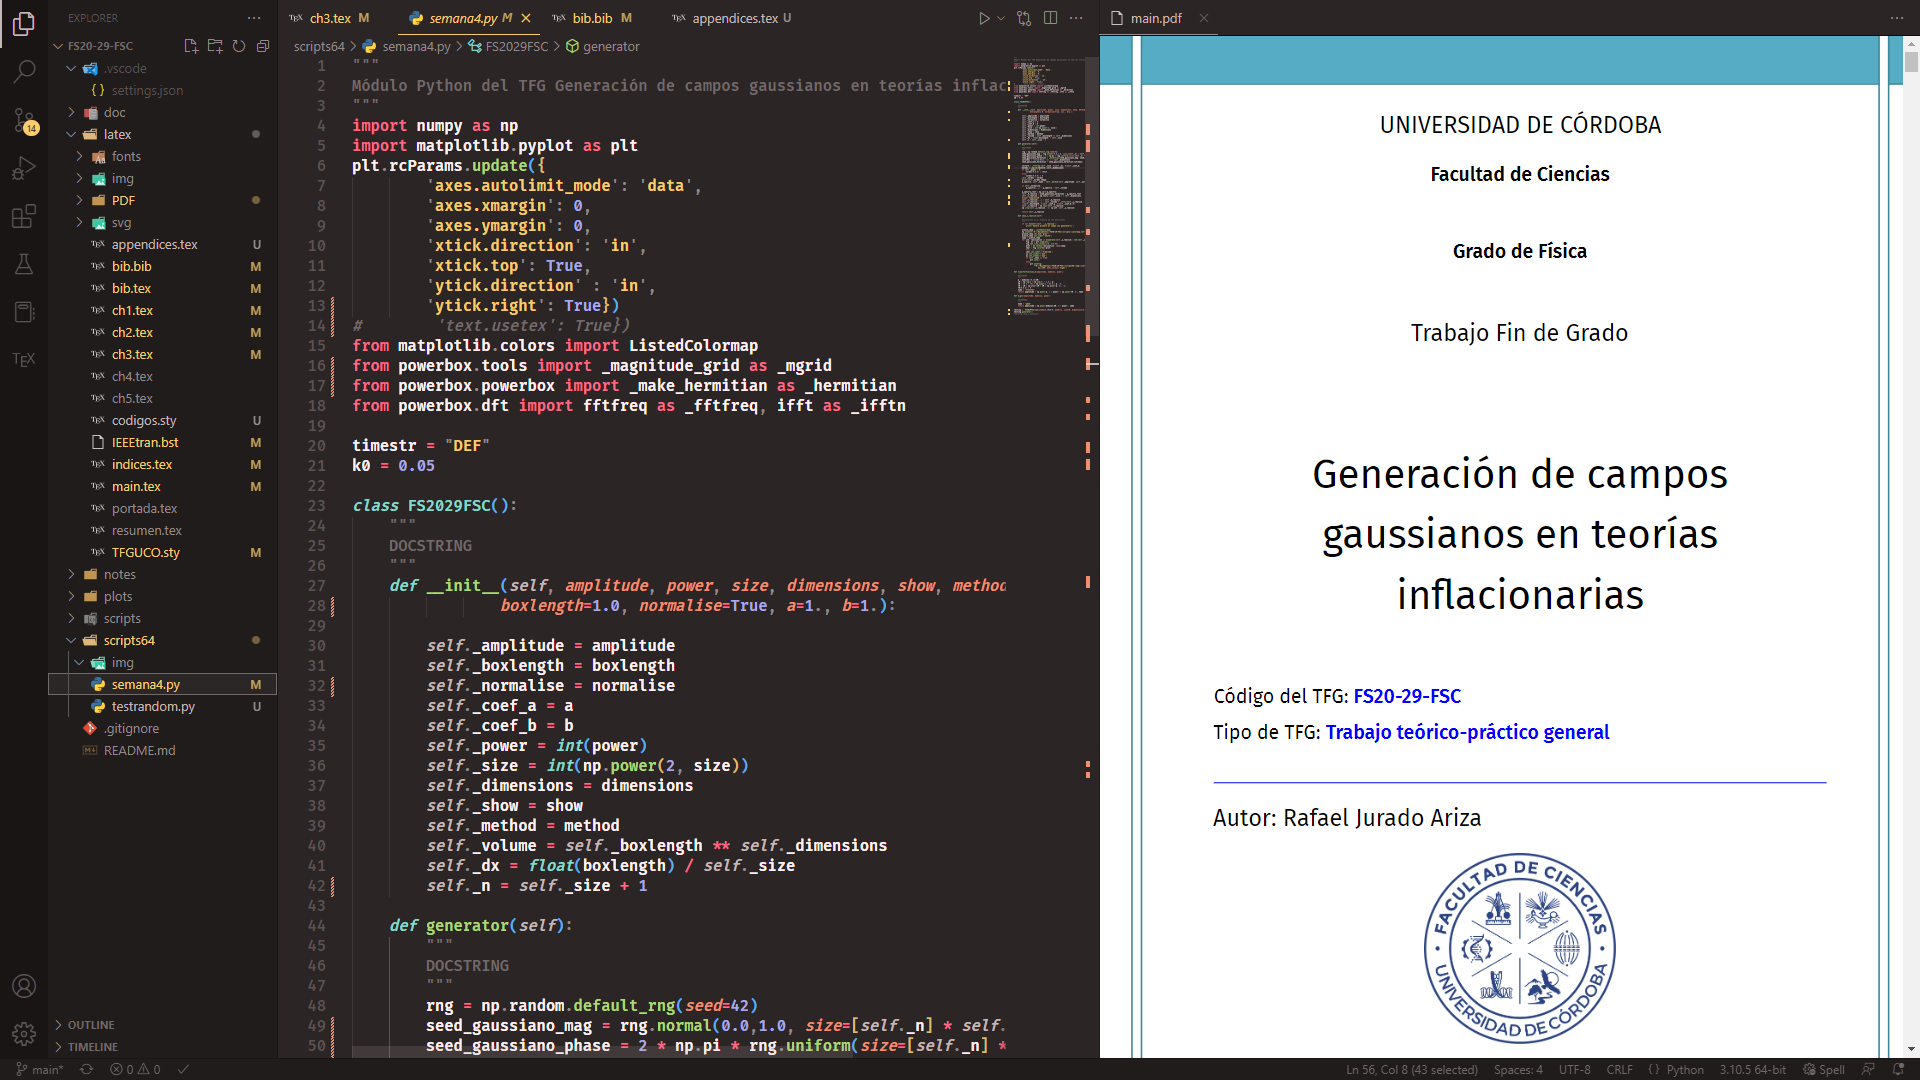
\includegraphics[width=\textwidth]{img/entorno.png}
    \caption{Entorno de trabajo en VSCode}
    \label{fig::entorno}
\end{figure}
\subsection{Gráficos}
El último material utilizado, no menos importante, fue la librería Matplotlib~\cite{Hunter2007} de Python para generar las representaciones visuales de las realizaciones del campo aleatorio gaussiano de las fluctuaciones.